\documentclass{standalone}

\usepackage{standalone}
\usepackage{tikz}
\usetikzlibrary{er,positioning, calc}

\begin{document}

	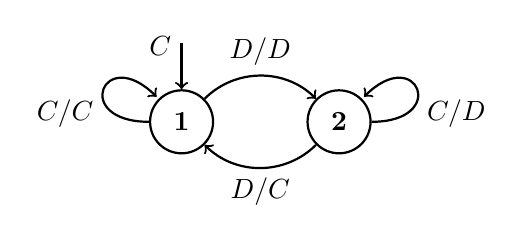
\begin{tikzpicture}
    	\tikzstyle{state}=[minimum width=0.8cm, font=\boldmath];


   	\node[circle, draw=black, thick] (0) at (0, 0) [state]    {$1$};
   	\node[circle, draw=black, thick] (1) at (2, 0) [state]   {$2$};

    	\coordinate (s) at (0, 1);

    	\draw (s) edge[out=-90, in=90, ->, thick] node [above left] {$C$} (0);
    	\draw (0) edge[out=180, in=135, ->, thick, loop] node [below left] {$C/C$} (0);
   	\draw (0) edge[out=45, in=135, ->, thick] node [above] {$D/D$} (1);

   	\draw (1) edge[out=-135, in=-45, ->, thick] node [below] {$D/C$} (0);
   	\draw (1) edge[out=0, in=45, ->, thick, loop] node [below right] {$C/D$} (1);

 
	\end{tikzpicture}
\end{document}